\documentclass[a4wide,10pt]{article}
\usepackage{a4wide}
\usepackage[applemac,utf8]{inputenc}
\usepackage[danish]{babel}
\usepackage[T1]{fontenc}
\usepackage{pdfsync}
\usepackage{amsmath,amssymb,amsfonts} 
\usepackage[pdftex]{graphicx}
\usepackage{wrapfig}
\usepackage{color}
\usepackage[small,bf]{caption}

\begin{document}
\title{DSB Portfolio 1}
\author{Nis Sarup}
\date{\today}
\maketitle

\section{Draw the double sided spectrum of the amplitudes for the signal x(t)} % (fold)
\label{sec:draw_the_double_sided_spectrum_of_the_amplitudes_for_the_signal_x_t_}
By using Eulers princible $x(t)$ can be rewritten as:
\begin{eqnarray}
	x(t)&=&2\cdot \frac{e^{i2\pi \cdot 1000t}+e^{i2\pi \cdot 1000t}}{2}+\frac{e^{i2\pi \cdot 3000t}+e^{i2\pi \cdot 3000t}}{2}+\frac{e^{i2\pi \cdot 19000t}+e^{i2\pi \cdot 19000t}}{2} \nonumber \\
	x(t)&=&e^{i2\pi \cdot 1000t}+e^{i2\pi \cdot 1000t}+\frac{1}{2} \cdot e^{i2\pi \cdot 3000t}+\frac{1}{2} \cdot e^{-i2\pi \cdot 3000t}+\frac{1}{2} \cdot e^{i2\pi \cdot 19000t}+\frac{1}{2} \cdot e^{-i2\pi \cdot 19000t}
\end{eqnarray}
Which gives us the coefficients:
\begin{eqnarray}
	c_1&=&1 \nonumber \\
	c_{-1}&=&1 \nonumber \\
	c_3&=&0,5 \nonumber \\
	c_{-3}&=&0,5 \nonumber \\
	c_{19}&=&0,5 \nonumber \\
	c_{-19}&=&0,5 \nonumber \\
\end{eqnarray}
And the double sided spectrum:
\begin{figure}[htbp]
	\centering
		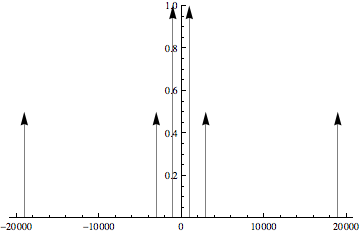
\includegraphics[width=8cm]{images/double-sided-spectrum-1.png}
	\caption{Double Sided Spectrum without aliasing}
	\label{fig:images_double-sided-spectrum-1}
\end{figure}

% section draw_the_double_sided_spectrum_of_the_amplitudes_for_the_signal_x_t_ (end)

\newpage

\section{Draw the double sided spectrum xs1(t) for the sampled signal without the
anti-aliasing filter} % (fold)
\label{sec:draw_the_double_sided_spectrum_xs1_t_for_the_sampled_signal_without_the_anti_aliasing_filter}
The samplerate of the A/D-converter is 20kHz. The new coefficients will be calculated by by multiplying them with the samplerate. Which gives:
\begin{eqnarray}
	c_1&=&20000 \nonumber \\
	c_{-1}&=&20000 \nonumber \\
	c_3&=&10000 \nonumber \\
	c_{-3}&=&10000 \nonumber \\
	c_{19}&=&10000 \nonumber \\
	c_{-19}&=&10000 \nonumber \\
\end{eqnarray}
And a plot of the double sided spectrum:
\begin{figure}[htbp]
	\centering
		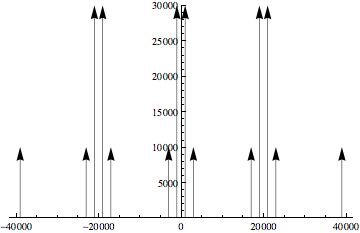
\includegraphics[width=8cm]{images/double-sided-spectrum-2.png}
	\caption{Double Sided Spectrum with aliasing}
	\label{fig:images_double-sided-spectrum-2}
\end{figure}
% section draw_the_double_sided_spectrum_xs1_t_for_the_sampled_signal_without_the_anti_aliasing_filter (end)
\newpage
\section{Calculate the A/D converter signal in dB} % (fold)
\label{sec:calculate_the_a_d_converter_signal_in_db}
A/D-converter signal can be calculated by using:
\begin{equation}
	SNR_{dB} = 10,79 + 20 \cdot Log_{10}(\frac{x_{rms}}{\Delta})
\end{equation}
Where:
\begin{equation}
	\Delta = \frac{x_{max} - x_{min}}{2^m}
\end{equation}
$x_{max}$ and $x_{min}$ is the maximum and minimum voltage for the A/D-converter and $m$ is the bitsize.
$x_{rms}$ is given by:
\begin{equation}
	x_{rms} = \sqrt{\frac{1}{T}\int_0^T x(t)^2 dT}
\end{equation}
We can then start calcualting:
\begin{eqnarray}
	x_{rms} &=& \sqrt{3} \nonumber \\
	\Delta = \frac{2 - (-2)}{2^8} &=& \frac{1}{64} \nonumber \\
	SNR_{dB} = 10,79 + 20 \cdot Log_{10}(\frac{\sqrt{3}}{\frac{1}{64}}) &=& 51,6848dB \nonumber
\end{eqnarray}
$SNR_{dB}$ is the strength of the signal.
% section calculate_the_a_d_converter_signal_in_db (end)

\end{document}